\subsection{Bestimmung der Gegenspannung}
Die Spektrallinien ist im folgenden so bezeichnet:
\begin{align}
	\text{rot:} \quad & \SI{615}{\nano\meter}
 \\
	\text{grün:} \quad & \SI{546}{\nano\meter}
 \\
	\text{lila:} \quad & \SI{435}{\nano\meter}
 \\
	\text{blau:} \quad & \SI{405}{\nano\meter}
 \\
	\text{UV:} \quad & \SI{365}{\nano\meter}
 \\
\end{align}
	
	
	
	
\begin{figure}[h!]
	\centering
	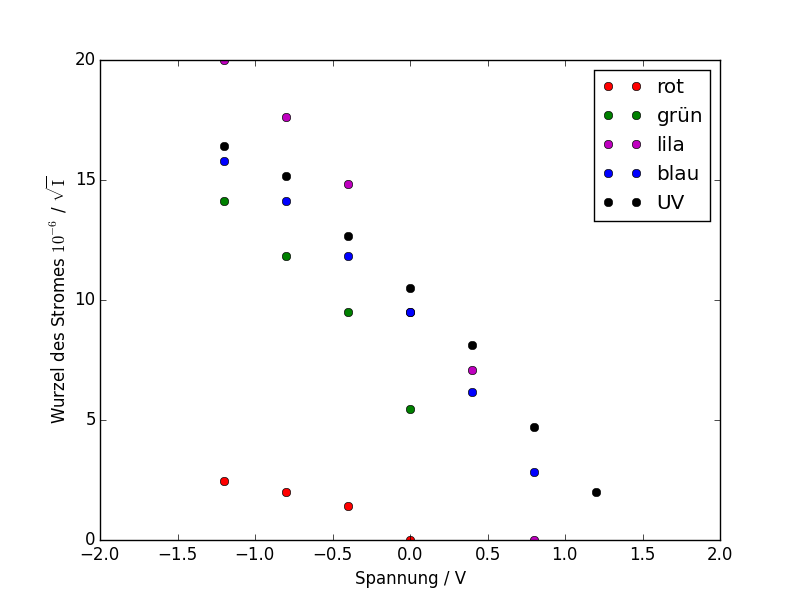
\includegraphics[width=0.7\textwidth]{build/AlleWellenlangen.png}
	\caption{gemessene Spektrallinien}
	\label{fig:spektrallinien}
\end{figure}

\begin{figure}[h!]
	\centering
	\captionof{table}{Gemessene elektrische Ströme / \si{\pico\ampere}}
	\begin{tabular}{c|ccccc}
		Spannung / V & rot & grün & lila & blau & UV \\
		\hline
		-2.00 & 8  & 260 & 600 & 350 & 360 \\
-1.60 & 6  & 240 & 520 & 280 & 300 \\
-1.20 & 6  & 200 & 400 & 250 & 270 \\
-0.80 & 4  & 140 & 310 & 200 & 230 \\
-0.40 & 2  & 90  & 220 & 140 & 160 \\
0.00  & 0  & 30  & 90  & 90  & 110 \\
0.40  & -1 & -20 & 50  & 38  & 66  \\
0.80  & -1 & -40 & 0   & 8   & 22  \\
1.20  & -1 & -40 & -4  & -2  & 4   \\
1.60  & -1 & -40 & -8  & -4  & -3  \\
2.00  & -1 & -40 & -10 & -5  & -5  \\

	\end{tabular}
	\label{tab:}
\end{figure}

\begin{figure}[h!]
	\centering
	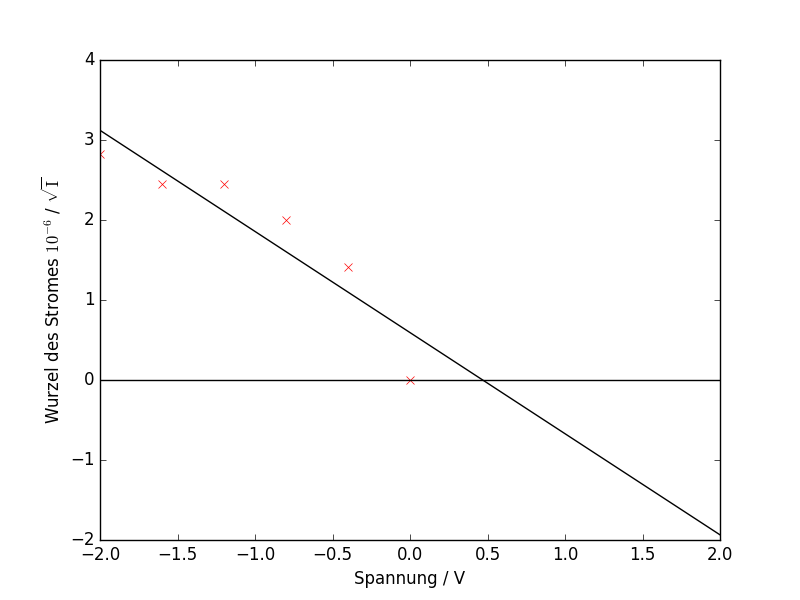
\includegraphics[width=0.7\textwidth]{build/regression_Farbe:0.png}
	\caption{Regression der roten Spektrallinie}
	\label{fig:regression_rot}
\end{figure}

\begin{figure}[h!]
	\centering
	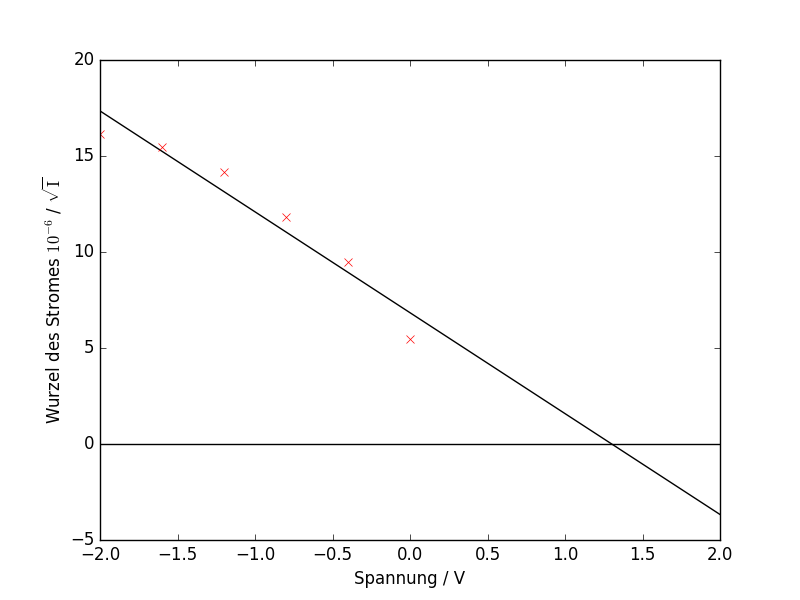
\includegraphics[width=0.7\textwidth]{build/regression_Farbe:1.png}
	\caption{Regression der grünen Spektrallinie}
	\label{fig:regression_grun}
\end{figure}

\begin{figure}[h!]
	\centering
	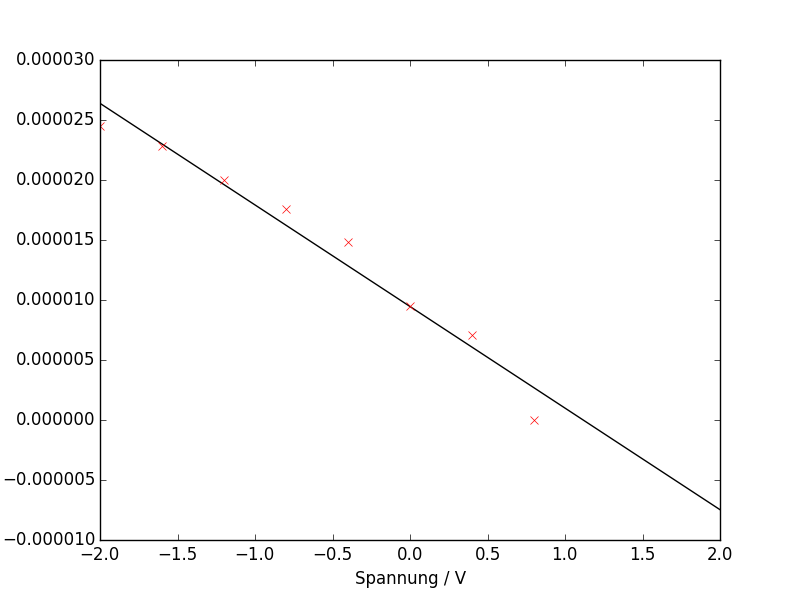
\includegraphics[width=0.7\textwidth]{build/regression_Farbe:2.png}
	\caption{Regression der lila Spektrallinie}
	\label{fig:regression_lila}
\end{figure}

\begin{figure}[h!]
	\centering
	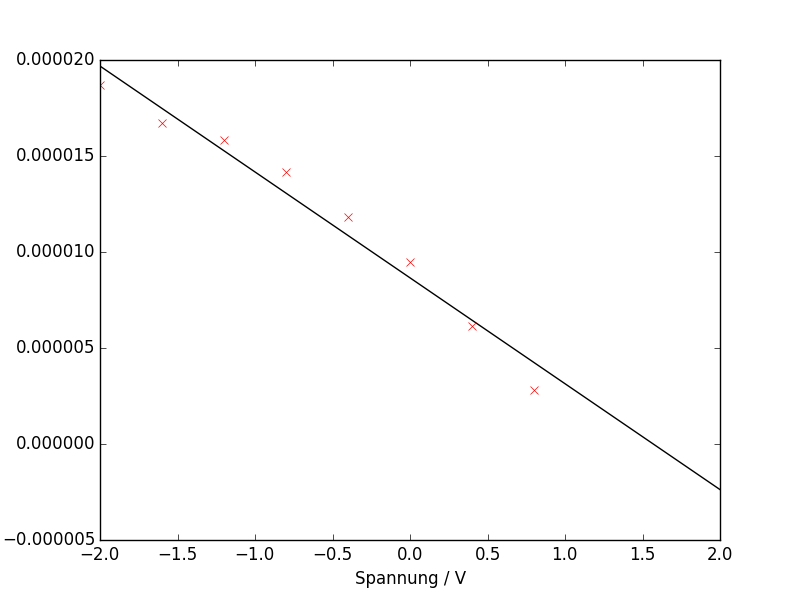
\includegraphics[width=0.7\textwidth]{build/regression_Farbe:3.png}
	\caption{Regression der blauen Spektrallinie}
	\label{fig:regression_blau}
\end{figure}

\begin{figure}[h!]
	\centering
	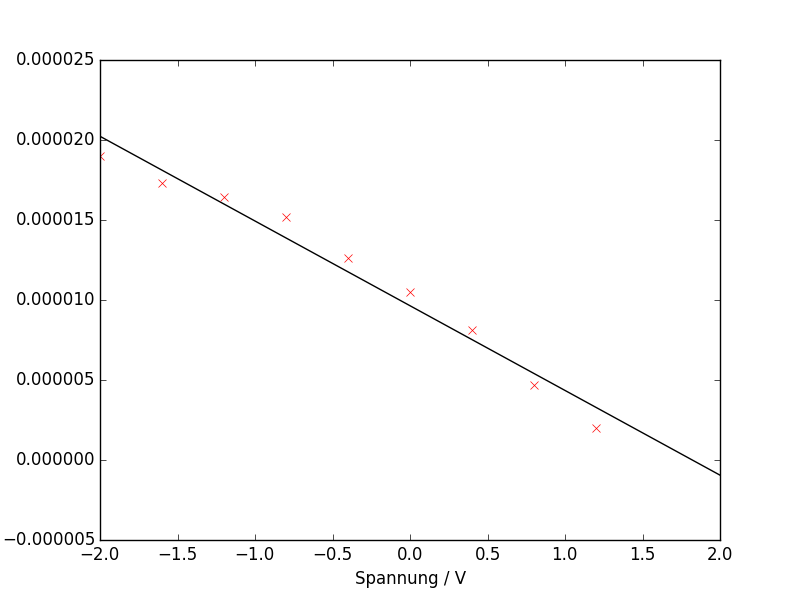
\includegraphics[width=0.7\textwidth]{build/regression_Farbe:4.png}
	\caption{Regression der ultravioletten Spektrallinie}
	\label{fig:regression_uv}
\end{figure}


\begin{align}
	\text{rot:} \quad m &= \SI{-0.00000126+-0.00000027}{\sqrt{\ampere}\per\volt}
 \\
		b &= \SI{0.00000059283+-0.00000033096}{}
 \\
		U_g &= \SI{0.46897+-0.28076}{\volt}
 \\
	\text{grün:} \quad m &= \SI{-0.00000525441+-0.00000068977}{\sqrt{\ampere}\per\volt}
 \\
	b &= \SI{6.0+-0.5}{\sqrt{\pico\ampere}}
 \\
	U_g &= \SI{1.30139+-0.23337}{}
 \\
	\text{lila:} \quad m &= \SI{-8.5+-0.7e-6}{\sqrt{\ampere}\per\volt}
 \\
	b &= \SI{0.00000945765+-0.00000072853}{\sqrt{\ampere}}
 \\
	U_g &= \SI{1.12+-0.12}{\volt}
 \\
	\text{blau:} \quad m &= \SI{-5.5+-0.4e-6}{\sqrt{\ampere}\per\volt}
 \\
	b &= \SI{8.7+-0.3}{\sqrt{\pico\ampere}}
 \\
	U_g &= \SI{1.3+-0.1}{\volt}
 \\
	\text{UV:} \quad m &= \SI{-0.00000529491+-0.00000034715}{\sqrt{\ampere}\per\volt}
 \\
	b &= \SI{9.6+-0.4e-6}{\sqrt{\ampere}}
 \\
	U_g &= \SI{1.82107+-0.13974}{}

\end{align}


